
\label{sect:photoz}

We evaluate the results of our template training algorithm by using our learned templates to estimate photo-z's for the test set of galaxies using the software package \bpz\ \citep{Benitez2000a}.
The test set consists of 20,496 galaxies (20\% of the total set), with mean redshift $z_\text{mean} = 0.69$, max redshift $z_\text{max} = 3.61$, and magnitudes $13.8 < i < 25.7$.
See Table \ref{tab:data_sets} for a full summary and Figure \ref{fig:redshift_dist} for the redshift distribution.

\subsection{Bayesian Photometric Redshifts}
\label{sect:bpz}

Bayesian Photometric Redshifts (\bpz; \citealt{Benitez2000a}) is a template-based photo-z estimator.
Template-based estimators take a set of SED templates, assumed to be spanning and exclusive, and calculate observed fluxes over a grid of redshift values. 
Each set of observed fluxes is then matched to a specific template and redshift determined to be the most likely to have produced the observed colors. 

For each template, \bpz\ evaluates a $\chi^2$ function at each redshift on the grid:
\begin{align}
    \chi^2 (z,T,A) = \sum_n \frac{1}{\sigma_n^2} (\, A \, \hat{f}_n(z,T) - f_n \,)^2,
    \label{eq:chi2}
\end{align}
where $T$ denotes the template, $z$ denotes the redshift, $A$ is a normalization, and $\hat{f}_n$, $f_n$, and $\sigma_n$ denote the calculated flux, the observed flux, and the fractional error as in Equation \ref{eq:cost_function}. 
The sum over $n$ is a sum over the filters for the set of observed fluxes. 
\bpz\ then evaluates the likelihood for producing the observed galaxy fluxes: $p(\{f_n\}|z,T) \propto \exp{(-\chi^2/2)}$. 
The redshift posterior is then calculated by marginalizing over the set of templates:
\begin{align}
    p(z|\{f_n\},m_0) &= \sum_T \, p(z,T|\{f_n\},m_0) \nonumber \\
                     &\propto \sum_T \, p(z,T|m_0) \, p(\{f_n\}|z,T),
\end{align}
where $p(z,T|m_0) = p(T|m_0) \, p(z|T,m_0)$ is a Bayesian prior over the apparent magnitude $m_0$. 
Work is underway to determine how best to use the full information encoded in the redshift posterior generated by \bpz\ and other photo-z codes (\note{cite examples of this}). 
In this work, however, only the peak of the posterior distribution is used to estimate the photo-z.

We use \bpz-v1.99.3\footnote{\url{http://www.stsci.edu/~dcoe/BPZ/}} \citep{Benitez2000a} to estimate photo-z's, providing the various sets of templates described in Section \ref{sect:application}.
We linearly interpolate two templates between each basis template, sorted by rest $u-g$ color, by setting \texttt{INTERP=2}. 
We use the default \bpz\ prior, which requires each SED template be broadly classified as either elliptical, spiral, or irregular/starburst. 
The SED classifications for each template set are discussed in Section \ref{sect:classification}. 
We use the one of the $i$ bands for the magnitude prior, in the following order of priority: $i$, $i_2$, $I$, $i^+$.
For simplicity, we treat non-detections as non-observations.
All other settings were left as default.

\bpz\ provides two metrics for the photo-z estimates: \texttt{ODDS} and $\chi_{\text{mod}}^2$.
\texttt{ODDS} measures how narrowly peaked the posterior distribution $p(z|\{f_n\},m_0)$ is around the estimated photo-z.
Galaxies with low \texttt{ODDS} have either broad redshift posteriors, or posteriors with multiple peaks.
$\chi_{\text{mod}}^2$ measures how well the best fit template at the predicted redshift matches the observed fluxes. 
For more about these metrics, see Section 4 of \citet{Benitez2000a} and Section 4.3 of \citet{Coe2006a}.
In this work, photo-z estimates with \texttt{ODDS} $< 0.95$ or $\chi_{\text{mod}}^2 > 1$ are excluded from the analysis, and the fraction excluded on this bases is reported as $f_\text{cut}$.

To further evaluate the results of \bpz, we calculate the scatter, bias, and outlier fraction of the photo-z estimates. 
Photo-z estimates are known to be contaminated with a significant number of outliers.
This is largely driven by a degeneracy wherein the 1000\AA\ Lyman break in a high redshift galaxy spectrum is shifted to the position of the 4000\AA\ Balmer break in a low redshift galaxy spectrum. 
\bpz\ attempts to break this degeneracy with the galaxy magnitude prior (i.e. galaxies with brighter apparent magnitudes are more likely to be at a lower redshift), yet there are still a large number of outliers.

To address this issue, we evaluate the statistics of the interquartile range (IQR) of the data, as these measures are known to be robust to the presence of outliers.
We follow \citet{Graham2018a} in introducing the quantity $\Delta z_{1+z} = (z_{spec} - z_{phot})/(1 + z_{phot})$.
The numerator quantifies the photo-z error, and the denominator compensates for the larger uncertainty at high redshifts. 
We define the scatter of the photo-z estimates, $\sigma_\text{IQR}$,  as the width of the IQR in $\Delta z_{1+z}$, divided by 1.349 to convert to the equivalent of a Gaussian standard deviation. 
We define the bias of the photo-z estimates as the mean value of $\Delta z_{1+z}$ for galaxies within the IQR.
The uncertainties of these two values are bootstrapped by calculating the values on 1000 random samples with replacement. 
Outliers are identified as photo-z's with $\Delta z_{1+z} > 3 \sigma_{\text{IQR}}$, and the fraction of outliers is reported as $f_\text{out}$.

\note{Say something about template classification. Here is the previous blurb:
The Bayesian prior used by \bpz\ requires each of the SED templates be broadly classified as either elliptical, spiral, or irregular/starburst. 
To perform this classification, we compare the colors of the trained templates with the original CWW+SB4 templates, which are already classified. }



\subsection{Photo-z Results}
\label{sect:photoz_results}

We use our trained templates to estimate photo-z's for the galaxies in the validation set using \bpz\ \citep{Benitez2000a}, and evaluate the results by comparing to the spectroscopic redshifts and photo-z estimates using the original CWW+SB4 templates. 
\bpz\ was run with each of the template sets above, using the settings described in Section \ref{sect:bpz}, with the SED classifications listed in the preceding section. 

The photo-z results can be seen in Figure \ref{fig:photoz_results}.
The photo-z estimates that passed the cuts on \texttt{ODDS} and $\chi_\text{mod}^2$ are displayed as points: the inliers in blue, the outliers in orange.
The values of the photo-z statistics for each template set are printed in each panel.
By comparing the top two panels, one can see that the training algorithm decreases the outlier fraction, bias, and scatter of the photo-z results for the CWW+SB4 templates.
The bottom two panels show that similar results are obtained with the N8 and N16 template sets, demonstrating that this method can be used to generate photo-z templates without any a priori information about galaxy spectra.
Noticeably, the N8 and N16 sets perform considerably worse in the $z = 1.5$ to $z = 2.5$ range.
This behavior is generally expected of photo-z estimators, as the Balmer break leaves most band sets at around $z=1.4$ and the Lyman break does not enter most band sets until $z=2.5$.
However, this flaw is especially pronounced in the N8 and N16 sets as there is far less data for galaxies in this redshift range for the sets to train on (c.f. Figure \ref{fig:redshift_dist}).
This, together with the fact that the trained CWW+SB4 set performs the best, indicates that the training algorithm should be combined with spectral synthesis models and observed spectra to yield the best results over the widest redshift range.

The results for N8 and N16 are similar, indicating that the addition of further templates has minimal impact on photo-z estimation. 
In addition to these four template sets, we considered one additional ``augmented'' set, which consists of the 16 templates from N16, as well as the El, 25Myr, and 5Myr templates from CWW+SB4.
This set consists of 19 templates, and spans the widest range of the color space visible in Figure \ref{fig:color_classify} (i.e. it contains the N16 template set, plus the red template in the top right and the two blue templates in the bottom left in the right panel of Figure \ref{fig:color_classify}). 
These results were virtually indistinguishable from the N16 results, and are thus not displayed in Figure \ref{fig:photoz_results}.
This further supports the case that additional templates have little impact on photo-z's.

\begin{figure*}
    \centering
    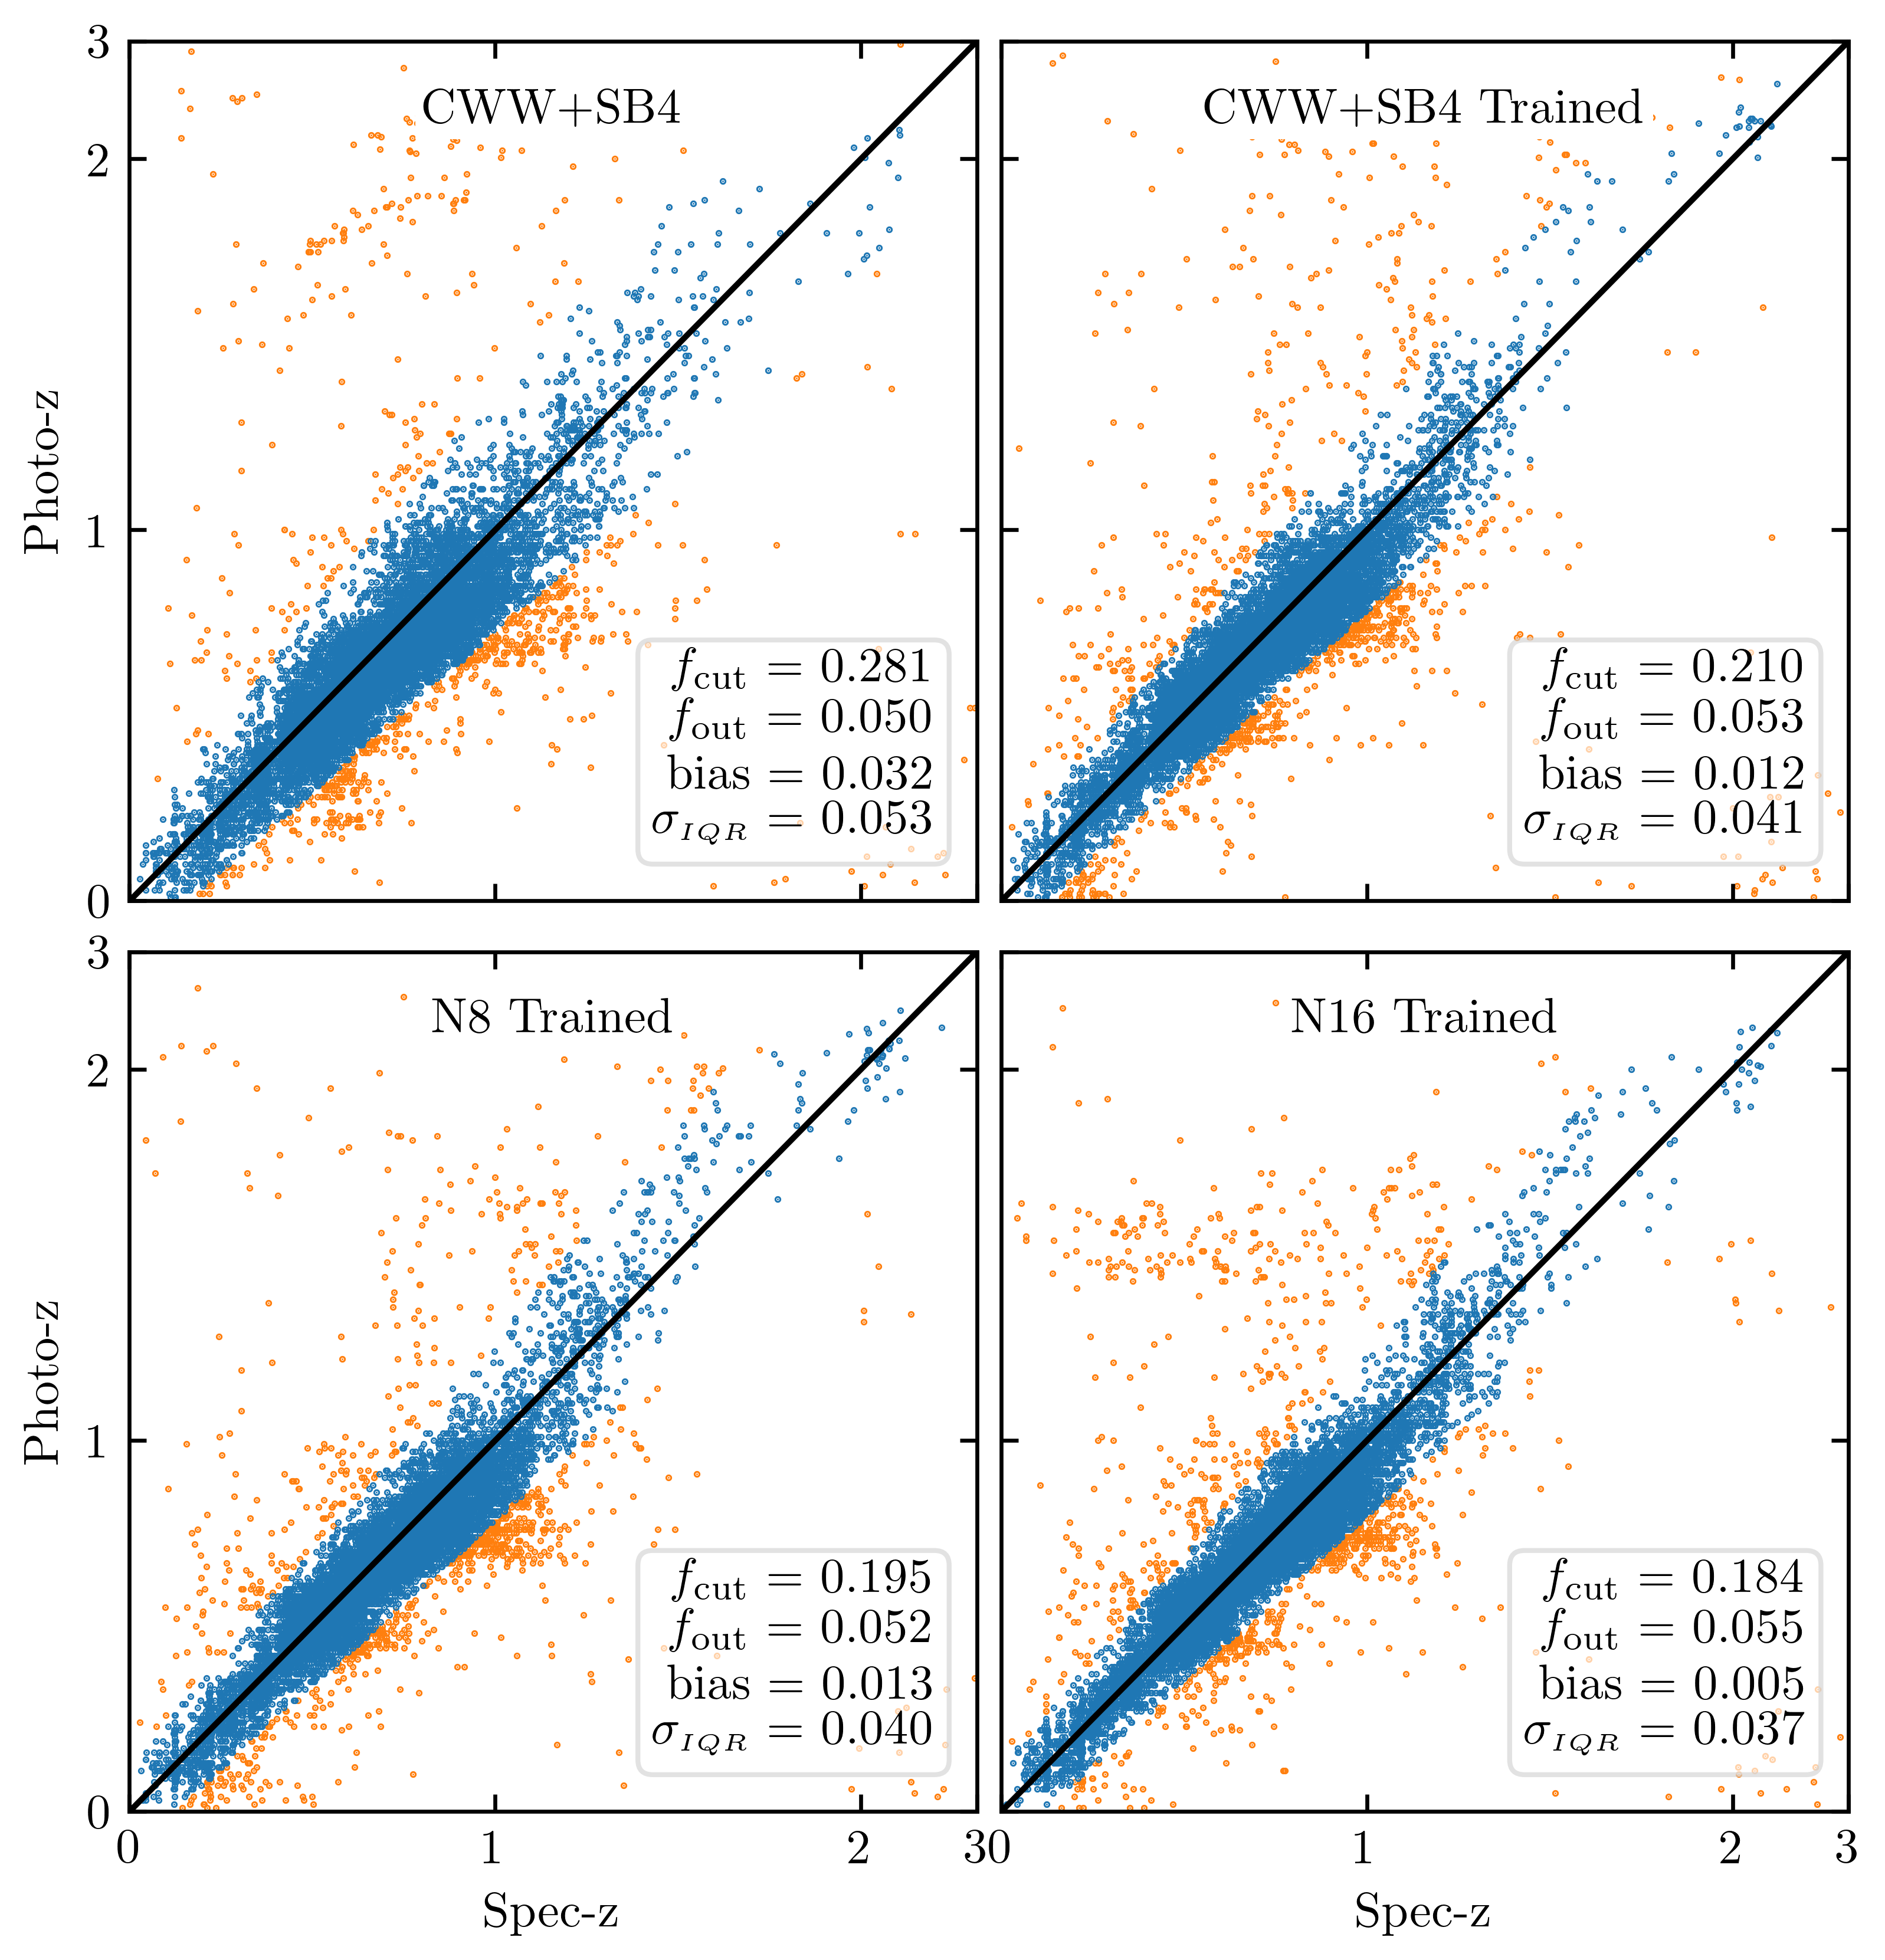
\includegraphics{photoz_results.png}
    \caption{Results of photo-z estimation with \bpz, using the four different templates sets. Photo-z estimates are displayed as points: inliers are blue and outliers are orange. The black line represents perfect estimation (i.e. photo-z = spec-z). The statistics printed in each panel are for the entire data set.}
    \label{fig:photoz_results}
\end{figure*}

The value of the metrics as a function of photo-z can be seen in Figure \ref{fig:photoz_binned}. For comparison, plotted in gray are the LSST science requirements for the metrics as listed in the LSST Science Requirement Document (SRD; \citealt{Ivezic2018}).
The SRD lists the following minimum requirements to enable the envisioned LSST cosmological studies: root-mean-square error $< 0.02(1+z_\text{phot})$; $f_\text{out} < 10\%$; average bias $<0.003(1+z_\text{phot})$.
The SRD lists these requirements for an $i<25$, magnitude-limited sample of four billion galaxies from $0.3 < z < 3.0$.
For comparison, our test set consists of 15,650 galaxies with $i < 27.4$, in the range $z < 3.3$, including 13,510 galaxies with $i < 25$, in the range $0.3 < z < 3.0$.
In Figure \ref{fig:photoz_binned}, you can see that our training algorithm goes a long way towards reaching the LSST goals for bias and scatter.

\begin{figure*}
    \centering
    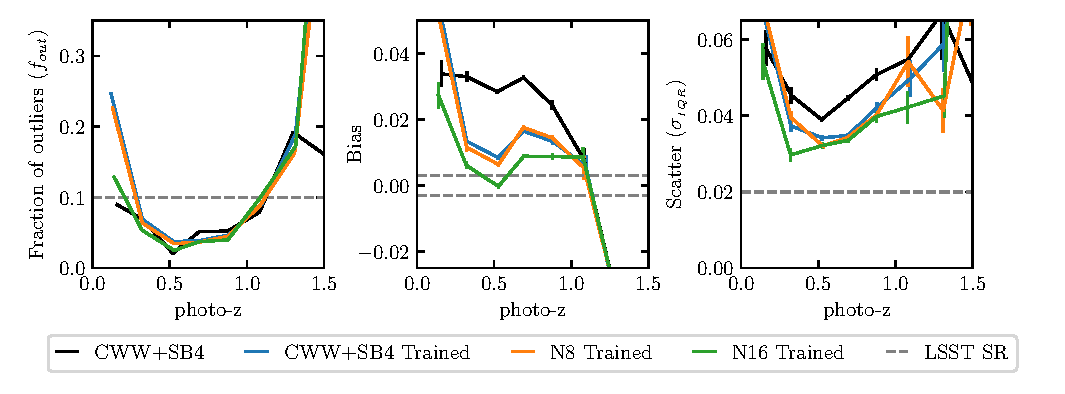
\includegraphics{figures/photoz_binned_metrics.pdf}
    \caption{Photo-z metrics as a function of redshift bin. LSST science requirements are displayed as dashed gray lines.}
    \label{fig:photoz_binned}
\end{figure*}